\pdfoutput=1

\documentclass[11pt]{article}

\usepackage{EMNLP2023}

\usepackage{times}
\usepackage{latexsym}
\usepackage[T1]{fontenc}
\usepackage[utf8]{inputenc}
\usepackage{microtype}
\usepackage{inconsolata}

\usepackage{booktabs}
\usepackage{adjustbox}
\usepackage{amsmath, amsfonts, amssymb}
\usepackage{graphicx}
\usepackage{multirow}
\usepackage{xcolor}
\usepackage{url}
\usepackage{dblfloatfix}

\renewcommand{\dbltopfraction}{0.95}
\renewcommand{\textfraction}{0.05}

\title{Localizing Hallucinations: Weakly Supervised Temporal\\ Uncertainty Quantification in LLM Activations}
\author{
  Javier Quiros\thanks{\,Corresponding author.}, Fatemeh Haji, Peyman Najafirad \\
  University of Texas at San Antonio \\
  \texttt{javier.delarosaquiros@utsa.edu}
}

\begin{document}
\maketitle

\begin{abstract}
Hallucinations in large language models (LLMs) pose significant reliability concerns, especially in long-form generations where supported and unsupported claims can appear within the same response. Recent work has shown that LLM internal representations contain useful signals for detecting hallucinations. However, mechanistic
detectors often miss signals distributed across tokens and layers.
Detecting hallucinations in long-form LLM outputs is challing because they often mix supported and unsupported claims, requiring detectors to localize unreliable spans rather than predicting a label for the entire response. Internal representations contain useful hallucination signals, but current mechanistic detectors rely on predetermined tokens or layers. Probes that use fixed layers or tokens miss signals from other positions. Probes that pool activations from the full-response learn global patterns not local ones. Claim extractors and classifiers miss signals before the hallucinated claim. We introduce Temporal Perception Encoder (TPE) that predicts hallucinations based on local signals within a window of tokens and signals from previous tokens.
We achieve this localization by training the model using multi-instance learning over token-centered windows of hidden-state activations. It uses claim or sequence level labes to learn to localize at the token level. Expriments on long-form outputs from biographical generation, open-ended factual QA, and retrieval-augmented QA show that TPE outperforms state-of-the-arts methods.
\end{abstract}

\section{Introduction}

\begin{figure}[!t]
\centering
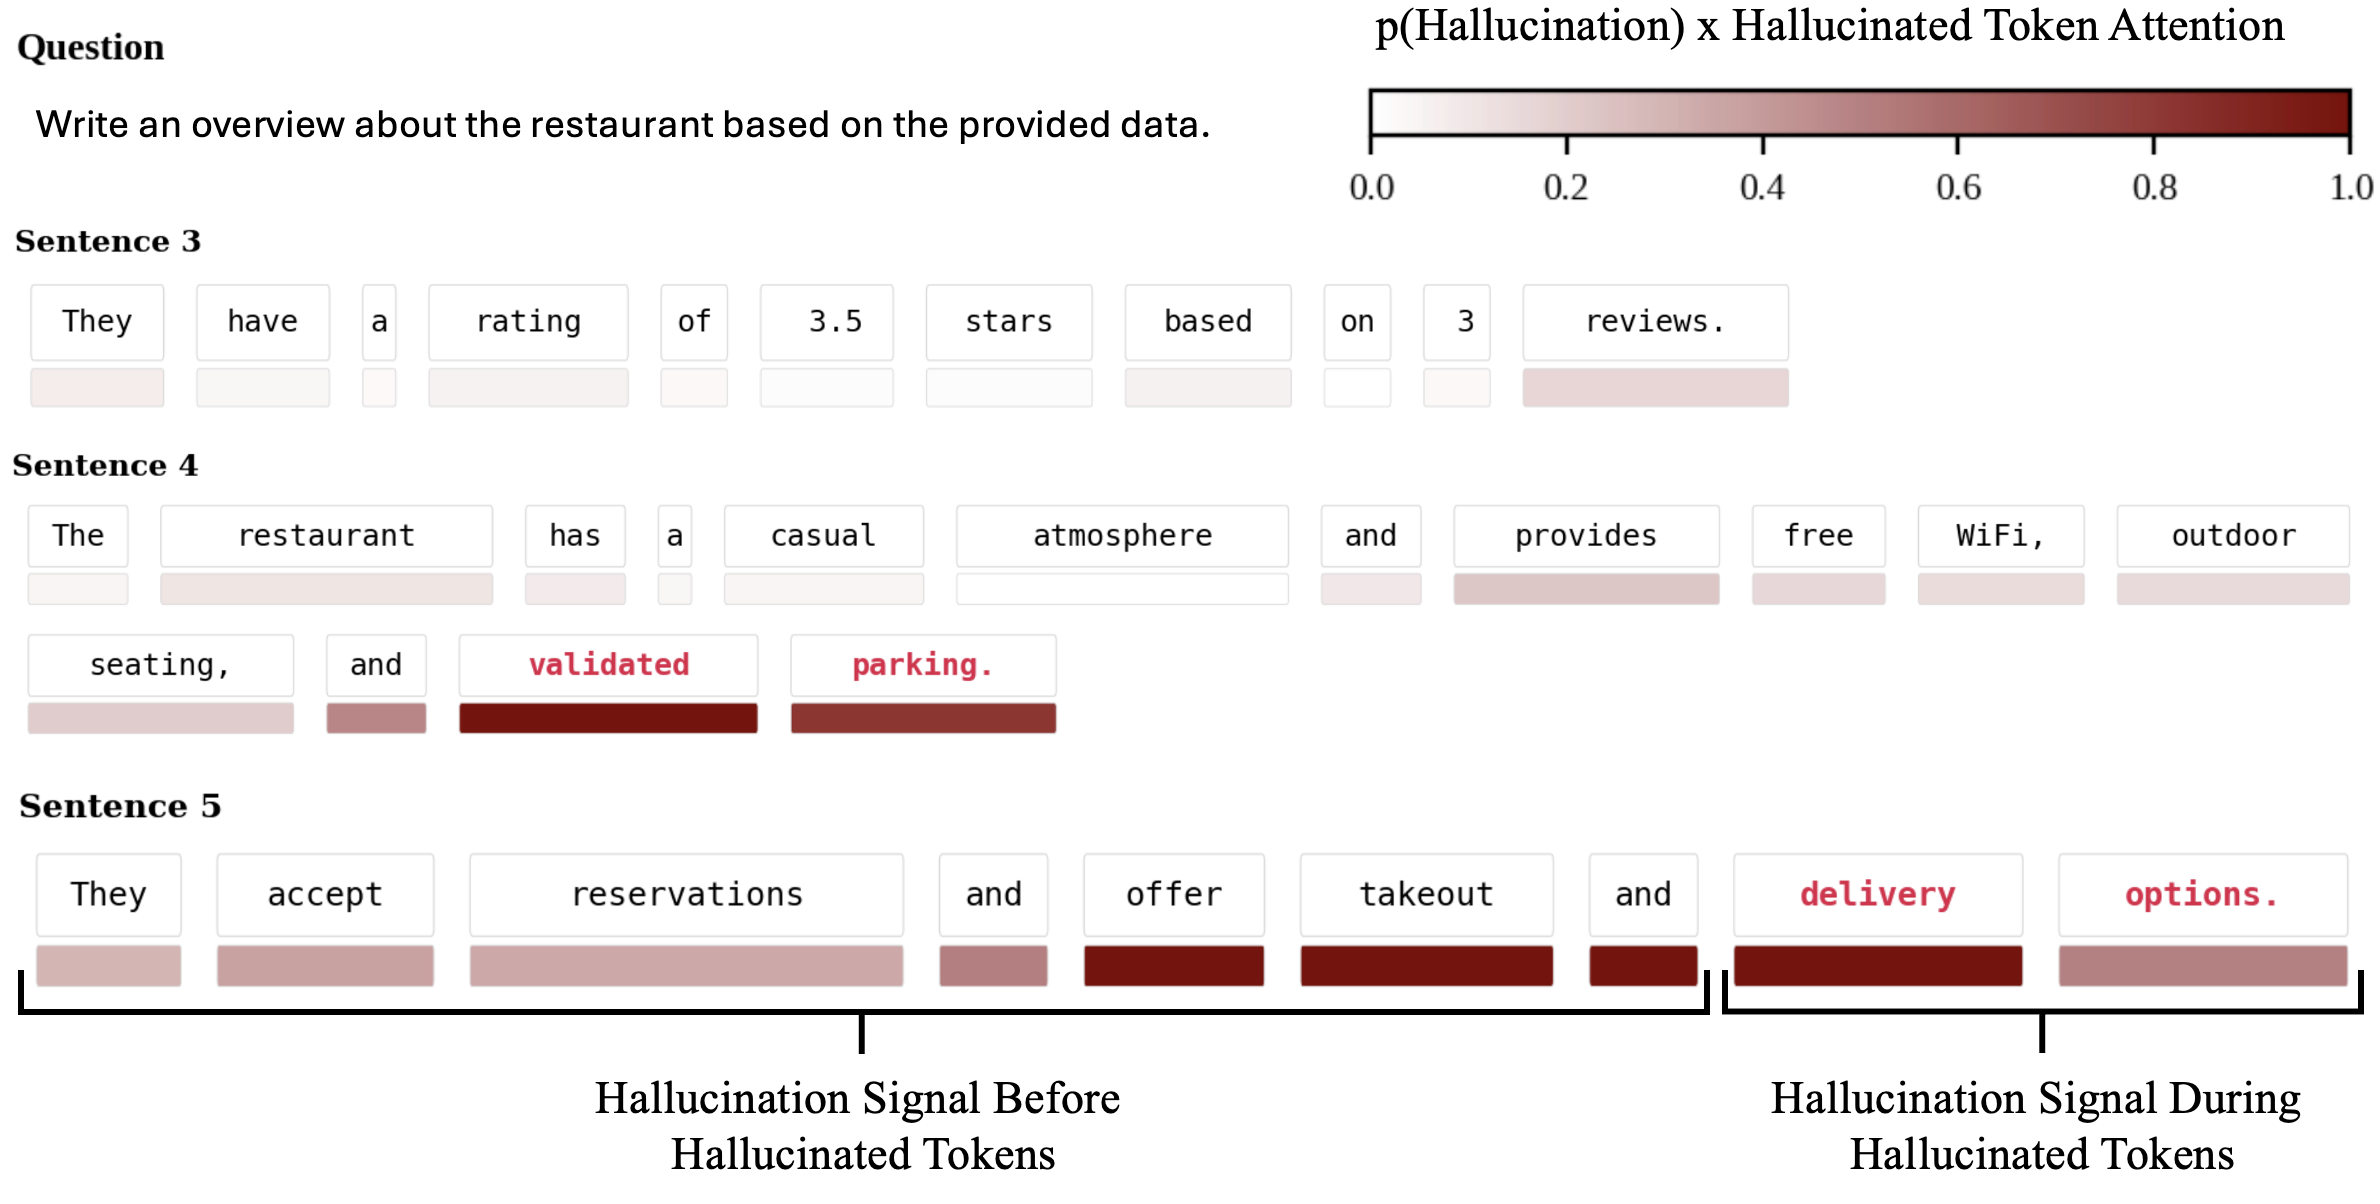
\includegraphics[width=\linewidth]{figs/tpe_example.png}
\caption{TPE on a generated sentence: per-token uncertainty signals from
the LLM's hidden states (top) are read by TPE and aggregated into
per-window hallucination scores (bottom), localizing the unsupported
span \emph{``in Alabama''} without per-token labels.}
\label{fig:tpe_example}
\end{figure}


\paragraph{Why this matters.}
Recent progress in large language models has demonstrated impressive capabilities in generating long-form answers across retrieval-augmented generation, biographies, and explanatory tasks.
However, their growing use also raises concerns about reliability, because fluent outputs can contain localized factual errors that are difficult to notice. A useful hallucination detector should identify where unreliable content appears, not just whether the full response is hallucinated. This distinction matters for retrieval-augmented answers, biographies, and long explanations, where a single unsupported span can be hidden inside otherwise correct text
\citep{niu2024ragtruth,min2023,wei2024}.

\paragraph{What current methods leave open.}
Confidence-based methods estimate uncertainty from sequence probabilities,
entropy, or related token statistics, but they do not directly model semantic
equivalence and often degrade on long-form generations
\citep{malinin2021uncertainty,duan2024shifting,schweighofer2025rethinking}.
Sampling-based methods compare several generations, and verifier pipelines
decompose responses into claims and check them with external systems
\citep{kuhn2023semantic,lin2024generating,jiang2024,manakul2023,min2023,zhao2024}.
These methods can be accurate, but repeated sampling, retrieval, or LLM-based
judging is expensive when applied across long passages. Mechanistic methods avoid
extra LLM calls by inspecting hidden states of the generating model
\citep{azaria2023,marks2023,liu2024,ji2024}, but each family hits a different
wall. Fixed layer-token probes are cheap but miss uncertainty signals that move
across layers, positions, models, and tasks \citep{kadavath2022,orgad2024}.
Full-response activation-map probes capture more distributed signal, but pooling
a whole response into one representation produces a sequence-level score and
forces a tradeoff between speed and accuracy as outputs grow longer
\citep{barshalom2025}. The common workaround is to extract claims, classify each
claim, and broadcast the verdict to the claim's text span, but this ignores
pre-span, post-span, and boundary evidence in the surrounding generation
\citep{snyder2024,he2024}.

\paragraph{Our approach and contributions.}
We recast mechanistic hallucination detection as weakly supervised temporal
localization (WSTL), borrowing from video understanding: a video model localizes
an action from clip-level labels without per-frame supervision
\citep{pilhyeonlee2021}. We treat hidden-state activations as a temporal sequence
over the generated token axis. Each instance is a fixed-length activation window
whose layer-token plane preserves local structure across layers and nearby
tokens. Figure~\ref{fig:tpe_example} shows the motivation for this windowed view:
hallucination evidence can appear before the unsupported tokens and influence
the hallucinated span. Based on this representation, we build Temporal Perception
Encoder (TPE): a Perception Encoder over local layer-token activation windows
paired with a temporal head that propagates window-level uncertainty evidence
across the response \citep{bolya2025perceptionencoder,albertgu2024}. Concretely,
we contribute:
\begin{enumerate}
    \item We formulate mechanistic hallucination detection as weakly supervised
    temporal localization over hidden-state activation windows, enabling predictions
    as granular as token level from claim labels.

    \item We propose TPE, a windowed hallucination detection model that encodes local
    layer-token activations with a Perception Encoder and propagates hallucination signals with
    a temporal head. We train it with a three-stage weak-supervision framework that learns
    hallucination activation patterns with claim labels, localizes responsible windows with
    top-$k$ MIL, and refines boundary behavior across neighboring correct and
    hallucinated claims.

    \item We demonstrate granular long-form hallucination localization on
    biographical generation, open-ended factual QA, and retrieval-augmented QA
    when using claim-level labels for training. 
    We also show it outperforms other methods on short-form and long-form QA, machine translation, and math
    even when using weaker sequence-level labels.
\end{enumerate}

\section{Related Work}

\paragraph{Uncertainty estimation for LLMs.}
Output-based estimators score uncertainty from a single sequence
through token-level probability, predictive entropy, length-normalized
scoring, or SAR
\citep{malinin2021uncertainty,duan2024shifting,schweighofer2025rethinking},
or from semantic agreement across multiple samples
\citep{kuhn2023semantic,lin2024generating,jiang2024,nguyen2025snne};
recent work trims the 5--20-generation cost with diversity-promoting
or beam-based proposals
\citep{aichberger2025sdlg,park2025diversity,fadeeva2026beams} and
folds in cross-model disagreement to catch confident errors
\citep{hamidieh2026crossmodel}. Both families exhibit systematic length
bias even after normalization
\citep{vashurin2025line,santilli2025lengthbias} and decouple uncertainty
from the model's internal state, which motivates \emph{mechanistic}
estimators that read hidden representations directly. A first wave of
probes treats a single layer--token slice as input and separates truth
from error in the residual stream
\citep{kadavath2022,azaria2023,burns2022,marks2023,li2024,ji2024,liu2024,chen2024,orgad2024}.
Subsequent work widens this slice along several complementary axes:
ACT-ViT \citep{barshalom2025} pools the full layer--token plane as an
activation image through a Vision Transformer; fact-probe pushes
detection to claim-level granularity
\citep{snyder2024,he2024,han2025factprobe}; attention-based variants
exploit cross-token focus patterns
\citep{li2025uqac,duan2024shifting,yuksekgonul2023,sriramanan2024attention,vazhentsev2025rauq};
and feature-gap methods compare representations across contexts to
expose epistemic uncertainty
\citep{bakman2025featuregaps,gottesman2024,slobodkin2023,simhi2024}.
The common limitation is one score per response (or one forward per
claim, Figure~\ref{fig:inference_time}), which dilutes the signal as
responses grow long (Figure~\ref{fig:perf_by_length});
Figure~\ref{fig:signal_propagation} shows that the relevant activation
signal extends across tokens on both sides of a hallucinated span --
the structural fact that motivates our windowed formulation.

\paragraph{Uncertainty in long-form generation.}
Long responses interleave correct and uncertain content, which
single-score detectors cannot localize. Decomposition is the standard
remedy: at the claim level via atomic-fact extraction
\citep{min2023,wei2024,zhao2024} or conformal claim-level prediction
\citep{mohri2024}; at the sentence level by re-applying
self-consistency per sentence \citep{manakul2023,band2024}; and at
the token level via per-token probes \citep{he2024,su2024}. The
trade-off is real: claim and sentence pipelines depend on an external
extractor and one model call per unit, while token-level methods are
the only ones compatible with real-time generation -- though noisier
when read in isolation. We make the token level usable in practice by
sharing computation across a window of tokens rather than scoring each
in isolation, and by training under weakly supervised temporal
localization.

\paragraph{Weakly-supervised temporal localization.}
Our localization mechanism follows WTAL in video understanding, where
only video-level labels are available and per-frame relevance must be
inferred. \citet{pilhyeonlee2021} cast WTAL as uncertainty modelling,
treating background frames as out-of-distribution and aggregating
per-frame scores with multiple-instance learning. The analogy with
hallucination detection is direct: only response-level labels are
available, yet per-window uncertainty must be inferred. We treat
generated tokens as the temporal axis and aggregate per-window logits
with top-$k$ MIL.

\begin{figure}[t]
\centering
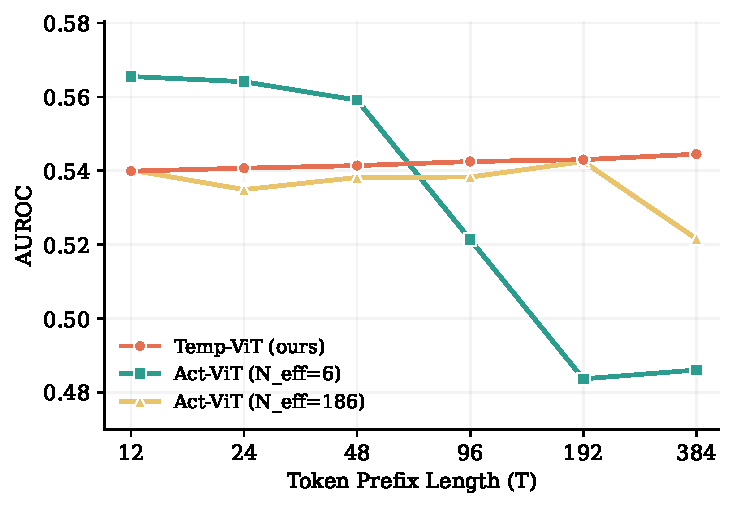
\includegraphics[width=0.95\linewidth]{figs/fig_perf_by_length.pdf}
\caption{Per-token AUROC on the LongFact prefix-truncation test as the
generated-token prefix length $T$ fed to each model grows. ACT-ViT
with its default short pooled token axis (\emph{Act-ViT, N\textsubscript{eff}=6})
peaks at short prefixes but collapses past $T = 48$ and falls below
chance for $T \in \{192, 384\}$ as the pooling compresses an
increasing number of token positions into the same fixed-size image.
Raising the pooled axis (\emph{Act-ViT, N\textsubscript{eff}=186})
partially rescues long prefixes but does not match Temp-ViT's flat
profile, which is per-token by construction. This illustrates the
long-form weakness of activation-tensor methods that pool the token
axis into a fixed-size representation.}
\label{fig:perf_by_length}
\end{figure}

\begin{figure}[t]
\centering
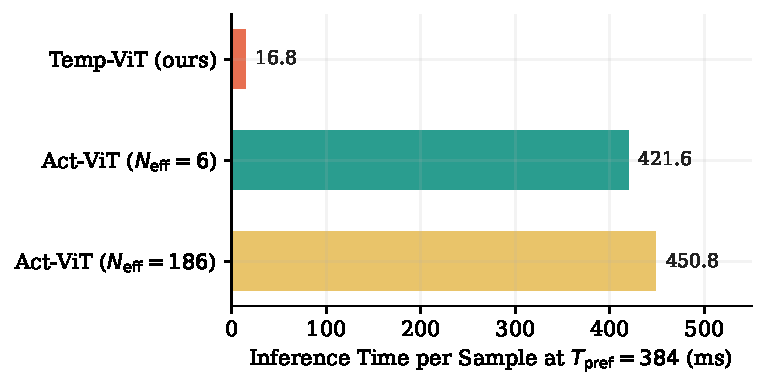
\includegraphics[width=0.95\linewidth]{figs/fig_inference_time.pdf}
\caption{Wall-clock time to score every token of one $T = 384$-token
LongFact passage on a single H200, batch~1, FP32. ACT-ViT emits one
scalar per call, so labelling every token requires $T$ sequential
forwards; per-call latency is small but the total scales linearly with
the response length, even when the post-pool ViT input is widened to
recover long-range accuracy (\emph{N\textsubscript{eff}=186}).
Temp-ViT produces the full per-token logit vector in a single forward
pass and is roughly $25\times$ faster on this passage, illustrating
the real-time-cost weakness of activation-tensor methods that need one
call per generated token.}
\label{fig:inference_time}
\end{figure}


\section{Towards Weakly Supervised Temporal Uncertainty Localization}
\label{sec:non_static}

Mechanistic detectors face a tension among coverage, localization,
and scalability. Fixed-position probes \citep{azaria2023,orgad2024}
are efficient but read only one layer-token slice, so they miss
signals that appear elsewhere in the activation tensor. Full-response
activation maps cover broader structure, but pooling the whole
response produces a sequence-level score and scales poorly for
localization \citep{barshalom2025}. Claim-level detectors provide
coarser localization, but scoring extracted claims in isolation
ignores boundary evidence from neighboring supported and hallucinated
spans \citep{snyder2024,he2024}. TPE therefore uses local activation
windows as the inference unit: each score is tied to a bounded token
neighborhood, while still covering evidence before, during, and after
the labeled span. Appendix Figure~\ref{fig:signal_propagation} shows
that hallucination signal appears before, within, and after
hallucinated spans.

\paragraph{Why encode activations as 2D images?}
Per-layer and per-token probes show that useful hidden-state signal
is not concentrated in one fixed position. Informative regions spread
across both the layer and token axes, and the most predictive
layer-token cells shift across LLMs, as shown by the heatmaps in
Appendix~\ref{app:heatmaps}. TPE preserves this local layer-token
plane instead of using one fixed slice or one-axis pooling. Following
the activation-image view of ACT-ViT \citep{barshalom2025actvit}, it
encodes each local activation window with Perception Encoder features
\citep{bolya2025perceptionencoder}.

\paragraph{Weakly supervised temporal localization.}
This representation turns hallucination detection into weakly
supervised temporal localization. As in video localization, where
clip-level labels supervise event discovery over time
\citep{pilhyeonlee2021}, a response label or claim label supervises
a sequence of candidate activation windows without window-level
annotations. Section~\ref{sec:model} formalizes this view: TPE
encodes local layer-token windows, propagates evidence with a
temporal head, and uses top-$k$ MIL so sparse hallucination evidence
can be assigned to a small subset of windows.

\section{Method}
\label{sec:model}

\begin{figure*}[t]
\centering
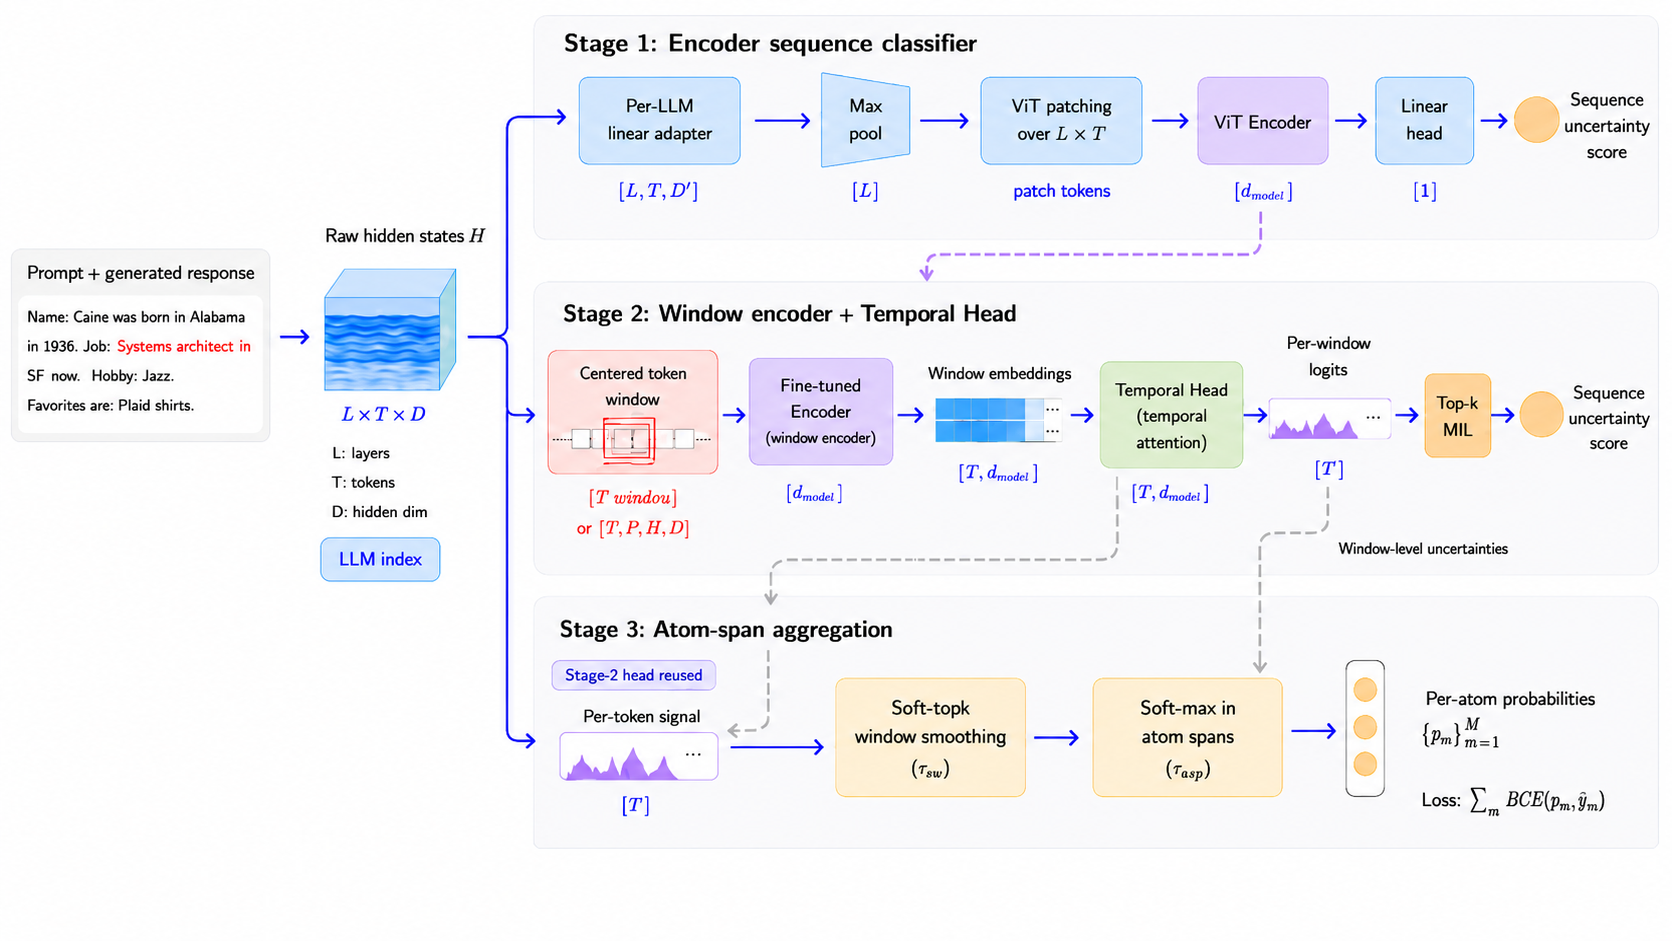
\includegraphics[width=0.95\linewidth]{figs/fig1_overview.png}
\caption{Three-stage Temp-ViT.
\textbf{Stage~1} (top): an ACT-ViT encoder maps a per-atom activation
tensor $A \in \mathbb{R}^{L \times T \times D}$ to an atom-level
uncertainty score via Pool $\to$ per-LLM linear adapter $\to$ ViT
$\to$ linear head.
\textbf{Stage~2} (middle): the encoder is frozen and applied to
centered length-$W$ token windows; a Mamba-2 temporal head emits one
logit per window, aggregated by top-$k$ MIL into an atom-level score.
\textbf{Stage~3} (bottom): the head is fine-tuned on whole passages
with noisy per-atom labels $\tilde{y}_m$ from atomic-fact
verification; per-token logits are smoothed and aggregated within
each atom span $(\ell_m, r_m)$ via a per-atom BCE, so the head ranks
uncertainty across atoms rather than scoring each in isolation.}
\label{fig:overview}
\end{figure*}


Figure~\ref{fig:overview} illustrates TPE's three-stage pipeline over
hidden-state activations $A \in \mathbb{R}^{L \times T \times D}$.
Stage~1 trains a sequence encoder $E_\theta$ on isolated labeled
segments, mapping $A$ to an embedding $e$ and sequence logit $z$.
Stage~2 slices the same activation tensor into centered length-$W$
windows $A^{(1)},\ldots,A^{(T)}$, adds a Mamba-2 temporal head
\citep{albertgu2024}, and trains per-window logits
$\hat{z}^{(1)},\ldots,\hat{z}^{(T)}$ through a top-$k$ MIL sequence
loss. Stage~3 freezes $E_\theta$ and refines the temporal head on
whole passages using claim spans $(\ell_m,r_m)$ and auxiliary labels
$\tilde{y}_m$, so the same token-window scores can be aggregated to
sentence, claim, and sequence predictions.

\subsection{Problem setup and notation}
\label{sec:notation}

Given an LLM $M$ and a generated response of length $T$, we collect
hidden-state activations $A \in \mathbb{R}^{L \times T \times D}$
over $L$ layers and hidden dimension $D$. For localization, TPE also
uses the windowed view
$A^{(t)} \in \mathbb{R}^{L \times W \times D}$, a length-$W$ slice
centered at generated position $t$. Training examples provide a
sequence label $y \in \{0,1\}$, and long-form corpora additionally
provide noisy claim labels
$\{(\ell_m, r_m, \tilde{y}_m)\}_{m=1}^{M}$ from claim-level
verification. The model predicts a sequence uncertainty score
$\hat{p}$ and per-window scores
$\{\hat{p}^{(t)}\}_{t=1}^{T}$; extended notation, dataset
construction, white-box assumptions, and off-domain generalization
are deferred to Appendix~\ref{app:extended}.

\subsection{Stage 1: Encoder}
\label{sec:act_vit_subsec}

The encoder has three components. Pool applies adaptive
max-pooling over $(L, T)$ to a target spatial size $(L_p, T_p)$,
yielding $A_p \in \mathbb{R}^{L_p \times T_p \times D}$. LA
is a per-LLM linear adapter
$LA_M : \mathbb{R}^D \to \mathbb{R}^{D'}$ that aligns hidden
dimensions across models, motivated by recent evidence that LLM
representations can be put in
approximate correspondence by linear maps
\citep{huh2024,moschella2022,kornblith2019}. The Perception Encoder
processes the pooled $(L_p \times T_p)$ activation image as a visual
input and returns a dense embedding for the layer-token plane
\citep{bolya2025perceptionencoder}. A linear head emits the Stage-1
logit $z$, trained with
$\mathcal{L}_{1} = \mathrm{BCE}(\sigma(z), y)$ where $y$ is the
sequence label; the pre-head features form the embedding reused by
Stages 2 and 3.

\subsection{Stage 2: Temporal Localization with Top-$k$ MIL}
\label{sec:temporal_head}

For each generated position $t$, we extract the windowed activations
$A^{(t)} \in \mathbb{R}^{L \times W \times D}$ as $W$ token
columns of $A$ centered at $t$. The same Pool is reused with a
smaller token target $(L_p, W_p)$, and $E_\theta$ produces a
per-window embedding $e^{(t)} \in \mathbb{R}^{d}$. Stacking the $T$
windows yields $E \in \mathbb{R}^{T \times d}$. A residual stack of
Mamba-2 blocks processes $E$ along the token axis followed by a
linear head:
$\hat{z}^{(t)} = h(\mathrm{Mamba\text{-}2}(E)_t)$.
Mamba-2's linear-time selective state-space recurrence makes Stage 2
viable for real-time streaming, where each new token requires only a
constant-memory update.

Because only sequence-level labels are
available, we train via top-$k$ MIL: after masking padded positions,
take the $k$ largest per-window logits and average them into one
sequence-level logit:
\begin{equation}
\hat{z} = \tfrac{1}{k}\!\!\!\sum_{t \in \mathrm{Top}_k(\{\hat{z}^{(t)}\}_t)}\!\!\!\hat{z}^{(t)}, \qquad \hat{p} = \sigma(\hat{z}),
\end{equation}
and supervise with $\mathcal{L}_{2} = \mathrm{BCE}(\hat{p}, y)$.
Mean-of-top-$k$ avoids the outlier sensitivity of max and the signal
dilution of a full mean while keeping the supervision sequence-level.

\subsection{Stage 3: Cross-Claim Refinement}
\label{sec:stage3}

Stages 1 and 2 see one claim segment at a time and do not observe
how the uncertainty activation signal changes across neighboring
claims. Mixed-content windows, whose receptive field straddles
hallucinated and supported tokens, combine signal regimes that
single-claim training cannot disentangle. Stage 3 therefore freezes
$E_\theta$ and fine-tunes the temporal head on whole passages with
claim spans $\{(\ell_m, r_m)\}_{m=1}^{M}$ and noisy labels
$\tilde{y}_m$. The Stage-2 detector emits passage-level per-token
logits, which are locally smoothed and aggregated within each claim
by a top-$k$ mean to form $\hat{z}_m$. A per-claim BCE loss
$\mathcal{L}_{3}$ trains the head to model the signal profile within
and across claims rather than scoring each claim in isolation; the
exact smoothing and claim aggregation are given in
Appendix~\ref{app:extended}.

At inference time, a single forward through the Stage-3 detector
yields the per-token logits over the whole passage, from which we
read off (i) the per-token / per-window scores
$\{\sigma(\hat{z}^{(t)})\}_{t=1}^{T}$ for token-level localization;
(ii) per-sentence scores obtained by aggregating the smoothed
per-token logits within each sentence span with the same top-$k$
mean; (iii) per-claim scores $\{\sigma(\hat{z}_m)\}_m$ when claims
are available; and (iv) a sequence-level score by reusing the
Stage-2 top-$k$ MIL aggregation.

\section{Experimental Setup}
\label{sec:experiments}

\subsection{Datasets}
\label{sec:datasets}

\paragraph{Hallucination detection.} For long-form hallucination
detection (Table~\ref{tab:main} and Appendix
Table~\ref{tab:token_level})
we evaluate on three corpora that anchor this task in recent work:
RAGTruth \citep{niu2024ragtruth}, a retrieval-augmented
generation corpus with span-level hallucination annotations across
QA, summarization, and data-to-text prompts;
FactScore \citep{min2023}, atomic-fact-verified biography
generations; and LongFact \citep{wei2024}, long-form factuality
prompts paired with the SAFE atomic-fact verifier of the same paper.
For each corpus we follow the original protocol to obtain per-claim
support labels and broadcast them to per-token labels via the
overlap-resolution rule of
Appendix~\ref{ablation:overlap_rule}, which the token-level eval
uses to break ties when two claim spans cover the same token. The
per-claim labels also serve as the auxiliary supervision signal
$\tilde{y}_m$ introduced in Section~\ref{sec:notation}.

\paragraph{Uncertainty quantification.} For sequence-level
uncertainty quantification (Table~\ref{tab:polygraph}) we use the
LM-Polygraph benchmark
\citep{fadeeva2023lmpolygraph,vashurin2025lmpolygraph}, following
\citet{vashurin2025lmpolygraph} for subset selection, prompt
formatting, and few-shot example sourcing. Quality measures are
accuracy for short-form QA (MMLU, GSM8k), AlignScore for long-form
QA (TriviaQA, CoQA), and COMET for translation (WMT14 Fr-En, WMT19 De-En).

\paragraph{LLMs.} All experiments use three instruction-tuned
open-weight LLMs:
Mistral-7B-Instruct-v0.2 \citep{albertqjiang2023} (Mis-7B-Inst),
Llama-2-13B-chat-hf \citep{touvron2023} (LlaMa-13B-Inst), and
Llama-3.1-70B-Instruct \citep{touvron2023} (LlaMa-70B-Inst). For
each LLM we collect post-residual hidden states across all
transformer layers and all generated tokens, yielding the
hidden-state activations
$A \in \mathbb{R}^{L \times T \times D}$ that drive our method
(Section~\ref{sec:notation}).

\subsection{Baselines}
\label{sec:baselines}
We organize baselines into three row bands that match
Tables~\ref{tab:main} and~\ref{tab:polygraph}, with token-level
results in Appendix Table~\ref{tab:token_level}. All baselines are run through the
LM-Polygraph evaluation infrastructure
\citep{fadeeva2023lmpolygraph,vashurin2025lmpolygraph} on identical
generations and gold quality measures; sequence-level scores are
re-applied per sentence or per token when needed.

\paragraph{Confidence.} Score uncertainty from the model's
next-token distribution over generated tokens, or combine confidence
signals with attention-based features:
Maximum Sequence Probability (the LM-Polygraph default),
Perplexity \citep{fomicheva2020unsupervised},
Mean Token Entropy \citep{fomicheva2020unsupervised},
Self-Certainty \citep{kang2025selfcertainty},
TokenSAR \citep{duan2023},
Mean Pointwise Mutual Information \citep{takayama2019pmi},
BoostedProbSequence \citep{dinh2025boostedprob},
Contextualized Sequence Likelihood (CSL) \citep{lin2024csl},
Attention Score \citep{sriramanan2024attention}, and
Recurrent Attention-based Uncertainty Quantification (RAUQ)
\citep{vazhentsev2025rauq}.

\paragraph{Mechanistic.} Read model internals (hidden states or
activation maps) rather than the output distribution alone:
Fact-Probe \citep{han2025factprobe},
Feature-Gaps \citep{bakman2025featuregaps},
HaMI \citep{niu2025hami}, an MIL-based detector with
adaptive top-$k$ token selection and uncertainty-augmented
representations, and
Act-ViT \citep{barshalom2025}, the pooled-activation sequence
activation-map baseline.

\paragraph{Ours.} TPE is reported in two variants:
\emph{Encoder Only} -- the Stage-2 detector
(Section~\ref{sec:temporal_head}) used as a stand-alone per-window
scorer aggregated by top-$k$ MIL; and the full three-stage
\emph{TPE} pipeline (Section~\ref{sec:stage3}). Both are
trained with PRR as the validation criterion, following the
LM-Polygraph protocol.

\paragraph{Evaluation Measure.}
We report AUROC as the primary metric in
Table~\ref{tab:main}, Appendix Table~\ref{tab:token_level}, and
the Prediction Rejection Ratio
\citep{malinin2021uncertainty} for
Table~\ref{tab:polygraph}:
\begin{equation}
    \mathrm{PRR} = \frac{\mathrm{AUC}_{\mathrm{unc}} - \mathrm{AUC}_{\mathrm{rnd}}}{\mathrm{AUC}_{\mathrm{oracle}} - \mathrm{AUC}_{\mathrm{rnd}}},
    \label{eq:prr}
\end{equation}
which measures how well an uncertainty score ranks predictions by
quality relative to an oracle. We compute PRR up to a rejection
threshold of 50\%. AUROC, ECE, and Brier scores under the same
setup are reported in Appendix~\ref{app:extended}.

\paragraph{Generation setup.} All numbers are reported under
greedy decoding. Stochastic-sampling and best-sample variants
follow the LM-Polygraph defaults and are reported in
Appendix~\ref{app:extended}.

\section{Results}
\label{sec:results}

\subsection{TPE improves sentence-level hallucination localization}
\label{sec:results_aggregated}

The headline long-form result is sentence-level localization from
token-window predictions. TPE still emits one score per token window,
but Table~\ref{tab:main} reports sentence-level verdicts obtained by
aggregating those scores upward without retraining. We use the
sentence level as the main table because long-form labels come from
claim and atomic-fact verification pipelines: overlapping atoms can
assign noisy labels to individual tokens, while sentence aggregation
preserves the localized prediction task and reduces boundary noise.
Token-level results and the claim-span overlap rule are reported in
Appendix Table~\ref{tab:token_level} and
Appendix~\ref{ablation:overlap_rule}.

At the sentence level the Ours rows dominate every populated cell
except FactScore / LongFact for LlaMa-13B-Inst, where MeanTokenEntropy
edges out by 1--3 AUROC points. RAGTruth shows the cleanest
separation: TPE reaches $0.929$ sentence AUROC on
LlaMa-13B-Inst against the next-best baseline at $0.657$.
Sentence-length distributions
that determine which granularity is feasible to supervise are
reported in Table~\ref{tab:long_form_stats}; LongFact and
FactScore claims are typically much shorter than RAGTruth's,
which the per-token head benefits from at the sentence level.

\subsection{TPE outperforms baselines in uncertainty
quantification}
\label{sec:results_polygraph}

\begin{table*}[t]
\centering
\caption{Short-form uncertainty on the {\bf LM-Polygraph benchmark}
\citep{fadeeva2023lmpolygraph,vashurin2025lmpolygraph}. We report
AUROC per dataset over three task families: QA (TriviaQA, CoQA, MMLU,
GSM8k; binary accuracy), NMT (WMT14 Fr--En, WMT19 De--En; COMET
binarised at the training-set median), and summarization (XSUM;
AlignScore binarised at the training-set median). All methods are
evaluated under greedy decoding with the same generations and the same
gold quality measure. Methods are grouped by category:
\emph{Confidence} (sequence-level probability / entropy baselines),
\emph{Mechanistic} (model-internal signal baselines), and \emph{Ours}.
Best score per column is in \textbf{bold}; second-best is
\underline{underlined}. Cells with ``---'' indicate experiments not
yet run.}
\label{tab:polygraph}
\setlength{\tabcolsep}{2pt}
\renewcommand{\arraystretch}{1.05}
\scriptsize
\adjustbox{max width=\textwidth}{%
\begin{tabular}{l *{7}{c} *{7}{c} *{7}{c}}
\toprule
 & \multicolumn{7}{c}{Mis-7B-Inst} & \multicolumn{7}{c}{LlaMa-13B-Inst} & \multicolumn{7}{c}{LlaMa-70B-Inst} \\
\cmidrule(lr){2-8} \cmidrule(lr){9-15} \cmidrule(lr){16-22}
Method
  & TriviaQA & CoQA & MMLU & GSM8k & WMT14 & WMT19 & XSUM
  & TriviaQA & CoQA & MMLU & GSM8k & WMT14 & WMT19 & XSUM
  & TriviaQA & CoQA & MMLU & GSM8k & WMT14 & WMT19 & XSUM \\
\midrule
\multicolumn{22}{l}{\textit{Confidence}} \\
\cmidrule(l){1-22}
MaximumSequenceProbability
  & --- & --- & 0.3563 & 0.7403 & --- & 0.6796 & ---
  & --- & --- & ---    & ---    & --- & ---    & ---
  & --- & --- & ---    & ---    & --- & ---    & --- \\
Perplexity
  & --- & --- & 0.3563 & 0.6981 & --- & 0.7030 & ---
  & --- & --- & ---    & ---    & --- & ---    & ---
  & --- & --- & ---    & ---    & --- & ---    & --- \\
MeanTokenEntropy
  & --- & --- & 0.3554 & 0.7021 & --- & 0.7330 & ---
  & --- & --- & ---    & ---    & --- & ---    & ---
  & --- & --- & ---    & ---    & --- & ---    & --- \\
SelfCertainty
  & --- & --- & 0.3525 & 0.6610 & --- & 0.7766 & ---
  & --- & --- & ---    & ---    & --- & ---    & ---
  & --- & --- & ---    & ---    & --- & ---    & --- \\
TokenSAR
  & --- & --- & 0.5238 & 0.6963 & --- & 0.7013 & ---
  & --- & --- & ---    & ---    & --- & ---    & ---
  & --- & --- & ---    & ---    & --- & ---    & --- \\
MeanPointwiseMutualInformation
  & --- & --- & 0.8072 & 0.4533 & --- & 0.5470 & ---
  & --- & --- & ---    & ---    & --- & ---    & ---
  & --- & --- & ---    & ---    & --- & ---    & --- \\
BoostedProbSequence
  & --- & --- & 0.4072 & 0.7011 & --- & 0.7459 & ---
  & --- & --- & ---    & ---    & --- & ---    & ---
  & --- & --- & ---    & ---    & --- & ---    & --- \\
\midrule
\multicolumn{22}{l}{\textit{Mechanistic}} \\
\cmidrule(l){1-22}
CSL
  & --- & --- & 0.3349 & 0.7015 & --- & 0.6931 & ---
  & --- & --- & ---    & ---    & --- & ---    & ---
  & --- & --- & ---    & ---    & --- & ---    & --- \\
AttentionScore
  & --- & --- & 0.4954 & 0.4920 & --- & 0.5100 & ---
  & --- & --- & ---    & ---    & --- & ---    & ---
  & --- & --- & ---    & ---    & --- & ---    & --- \\
RAUQ
  & --- & --- & 0.4066 & 0.7128 & --- & 0.6561 & ---
  & --- & --- & ---    & ---    & --- & ---    & ---
  & --- & --- & ---    & ---    & --- & ---    & --- \\
FactProbe
  & --- & --- & ---    & ---    & --- & ---    & ---
  & --- & --- & ---    & ---    & --- & ---    & ---
  & --- & --- & ---    & ---    & --- & ---    & --- \\
Feature-Gaps
  & --- & --- & ---    & ---    & --- & ---    & ---
  & --- & --- & ---    & ---    & --- & ---    & ---
  & --- & --- & ---    & ---    & --- & ---    & --- \\
Act-ViT (F-v2, N\textsubscript{eff}=6)
  & --- & --- & \underline{0.9165} & \textbf{0.8643} & --- & 0.7775 & ---
  & --- & --- & ---    & ---    & --- & ---    & ---
  & --- & --- & ---    & ---    & --- & ---    & --- \\
\midrule
\multicolumn{22}{l}{\textit{Ours}} \\
\cmidrule(l){1-22}
Temp-ViT (Encoder Only)
  & --- & --- & 0.9108 & \underline{0.8604} & --- & \textbf{0.7989} & ---
  & --- & --- & ---    & ---    & --- & ---    & ---
  & --- & --- & ---    & ---    & --- & ---    & --- \\
Temp-ViT
  & --- & --- & \textbf{0.9214} & 0.8509 & --- & \underline{0.7835} & ---
  & --- & --- & ---    & ---    & --- & ---    & ---
  & --- & --- & ---    & ---    & --- & ---    & --- \\
\bottomrule
\end{tabular}%
}
\end{table*}


The LM-Polygraph benchmark
\citep{fadeeva2023lmpolygraph,vashurin2025lmpolygraph} stresses
the sequence-level use case: each test item is a short- or long-form
response and the goal is to rank responses by likely hallucination,
not to localize within them. Table~\ref{tab:polygraph} reports
per-category PRR on three capability categories of LM-Polygraph,
aggregated across the datasets present in each category for
Mis-7B-Inst: \emph{QA} (TriviaQA, CoQA, MMLU; today only MMLU
is filled), \emph{CoT} (GSM8k), and \emph{NMT} (WMT14, WMT19;
today only WMT19 is filled). The disaggregated per-dataset values
are reported in the ablation
Table~\ref{tab:polygraph_extended}. The Encoder Only row
aggregates per-window logits to a single number per response via
top-$k$ MIL, matching the training-time aggregator
(Section~\ref{sec:temporal_head}); the full TPE row uses the
Stage~3 passage-level head.

Encoder Only wins NMT ($0.816$) and slightly edges the Act-ViT
mechanistic baseline on QA ($0.114$ vs $0.113$). The full TPE
row loses some accuracy on the QA category: its Stage~3
objective is trained on long-form passages with many claims, and
the per-claim loss does not transfer back to single-claim
sequences as cleanly as the Stage~2 MIL objective. This is the
secondary contribution; the primary use case is localization
(Sections~\ref{sec:results_token}, \ref{sec:results_aggregated}),
but the per-token detector remains competitive as a sequence-level
ranker. Per-dataset sequence-length distributions are in
Table~\ref{tab:polygraph_stats}.

\subsection{Efficiency analysis}
\label{sec:results_efficiency}

TPE scores every generated token in a single forward through
the frozen encoder and the temporal head, so the cost of obtaining
sentence-level scores is amortized across the passage
rather than scaling with the number of claims.
Figure~\ref{fig:inference_time} quantifies this on a $T = 384$
LongFact passage: $25\times$ wall-clock advantage over
sequence-level pooled-activation baselines that must be re-invoked
per claim. Training the passage-level
refinement stage takes under three hours on a single H200 across
all three LLMs. Aggressive pooling
($(L_p, N_p) = (4, 20)$) preserves most of the downstream AUROC
while shrinking training to a few minutes.

\begin{figure}[t]
\centering
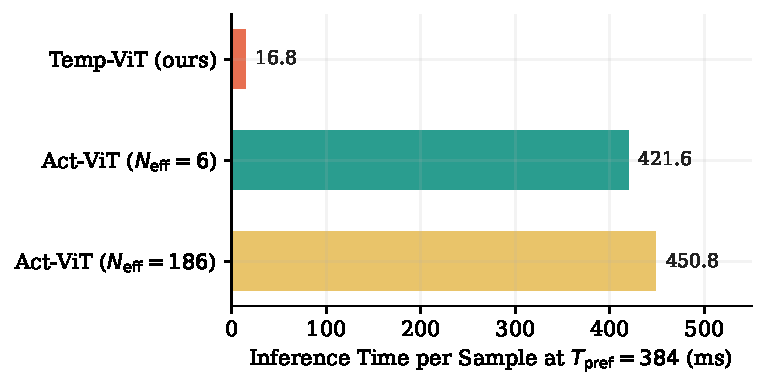
\includegraphics[width=0.95\linewidth]{figs/fig_inference_time.pdf}
\caption{Wall-clock time to score every token of one $T = 384$-token
LongFact passage on a single H200, batch~1, FP32. ACT-ViT emits one
scalar per call, so labelling every token requires $T$ sequential
forwards; per-call latency is small but the total scales linearly with
the response length, even when the post-pool ViT input is widened to
recover long-range accuracy (\emph{N\textsubscript{eff}=186}).
Temp-ViT produces the full per-token logit vector in a single forward
pass and is roughly $25\times$ faster on this passage, illustrating
the real-time-cost weakness of activation-tensor methods that need one
call per generated token.}
\label{fig:inference_time}
\end{figure}


\section{Conclusion}

We introduce TPE, a three-stage temporal uncertainty localization
framework that closes the long-form / real-time gap for mechanistic
hallucination detection. The encoder reads the full hidden-state
activations; the temporal head produces per-token logits under weakly
supervised top-$k$ MIL within each claim; the passage-level
refinement step turns those logits into per-claim scores that
discriminate uncertain claims from confident ones within the same
response. On RAGTruth, FactScore, and LongFact across three
instruction-tuned LLMs, the per-token output reaches token- and
sentence-level AUROC competitive with pooled-activation baselines while
running $25\times$ faster on long passages. On the
LM-Polygraph short-form benchmark, the same model produces a
sequence-level score plug-compatible with existing baselines. Promising
directions include richer attention-side features and shared per-LLM
adapters across model families.

\paragraph{Limitations.} The auxiliary span labels we train on are
noisy: claim-level verification pipelines mis-attribute hallucinated tokens to
neighbouring supported tokens, and the relevant activation signal can
fall outside the span (Appendix Figure~\ref{fig:signal_propagation}). The
Stage~3 BCE absorbs some of this noise but the per-claim numbers
still trail the encoder-only Stage~3 variant on the window ablation,
suggesting the temporal head over-fits to span boundaries when the
supervision is locally inconsistent. Our LLM-specific Linear Adapter
also assumes white-box access to hidden states and a small calibration
set per LLM; closed-weight settings remain out of scope. Finally, we
evaluate on English corpora and instruction-tuned chat models;
generalization to other languages and to base or reasoning-tuned
checkpoints is left for future work.


\bibliography{references}
\bibliographystyle{acl_natbib}

\appendix
\section{Ablations}
\label{sec:ablations}

\paragraph{Sentence- and claim-level results
(Tables~\ref{tab:sentence},~\ref{tab:claim}).} The same setup as
Table~\ref{tab:main}, reported at finer granularities: sentence-level
under AND-on-supported aggregation (any unsupported claim flips the
sentence) and one row per claim at the claim level. Temp-ViT (Stage~3)
outperforms the Act-ViT baseline at every populated cell, with the
gap widening as granularity narrows.

\paragraph{Architecture variants (Table~\ref{tab:window_ablation}).}
We compare the full Temp-ViT pipeline against an MLP-encoder baseline
(no windowing) and an encoder-only variant (no Mamba-2 head), across
the three stages. The encoder-only Stage~3 variant matches or beats
the full pipeline on AUROC on both RAGTruth cells, indicating that
the encoder's windowed pooling absorbs most of the local-context
signal; the temporal head's contribution comes from sequence-level
aggregation.

\paragraph{Stride (Table~\ref{tab:stride}).} We sweep the window
stride from 1 (the default, one window per token) to 4, 6, and
``no overlap'' (stride $=$ window size). Larger strides reduce
inference cost at the price of resolution.

\paragraph{Stages (Table~\ref{tab:stage}).} AUROC and PRR improve
monotonically from Stage 1 to Stage 3, with Stage 3 delivering the
largest gain on Llama-2-13b. The full per-stage table is provided on
two RAGTruth cells where stage-by-stage caches were available;
Mis-7B-Inst-v0.2 stage sweeps are pending.

\paragraph{Dataset statistics
(Tables~\ref{tab:long_form_stats},~\ref{tab:polygraph_stats}).}
Passage- and claim-length distributions help interpret which
granularities are feasible to supervise: LongFact and FactScore claims
are typically much shorter than RAGTruth's, which the per-token head
benefits from at sentence and claim levels.

\paragraph{Overlap (Table~\ref{tab:overlap}).} We sweep the four
combinations of overlapping vs.\ non-overlapping claim spans at
training and at test time. Non-overlapping span training is required
when claim spans share tokens; otherwise the head over-fits to the
longer-claim labels under the natural overlap.

\begin{table*}[t]
\centering
\caption{\textbf{Long-form hallucination detection --- sentence level.}
Same models, datasets, and metric as Table~\ref{tab:main}. Sentence
label uses AND-on-supported: any unsupported atom flips the sentence
to hallucinated; sentence score is the max per-token uncertainty in
the span. Best score per column in \textbf{bold}, second-best
\underline{underlined}. Cells with ``---'' indicate experiments not
yet run.}
\label{tab:sentence}
\setlength{\tabcolsep}{2.5pt}
\renewcommand{\arraystretch}{1.05}
\scriptsize
\adjustbox{max width=\textwidth}{%
\begin{tabular}{l ccc ccc ccc}
\toprule
 & \multicolumn{3}{c}{Mis-7B-Inst} & \multicolumn{3}{c}{LlaMa-8B-Inst} & \multicolumn{3}{c}{LlaMa-70B-Inst} \\
\cmidrule(lr){2-4} \cmidrule(lr){5-7} \cmidrule(lr){8-10}
Method & RAGTruth & FactScore & LongFact & RAGTruth & FactScore & LongFact & RAGTruth & FactScore & LongFact \\
\midrule
SemanticEntropy           & --- & --- & --- & --- & --- & --- & --- & --- & --- \\
DegMat (NLI)              & --- & --- & --- & --- & --- & --- & --- & --- & --- \\
EigValLaplacian (NLI)     & --- & --- & --- & --- & --- & --- & --- & --- & --- \\
SAR                       & --- & --- & --- & --- & --- & --- & --- & --- & --- \\
LUQ                       & --- & --- & --- & --- & --- & --- & --- & --- & --- \\
KernelLanguageEntropy     & --- & --- & --- & --- & --- & --- & --- & --- & --- \\
\midrule
Perplexity                & --- & --- & --- & --- & --- & --- & --- & --- & --- \\
MeanTokenEntropy          & --- & --- & --- & --- & --- & --- & --- & --- & --- \\
MCNSE                     & --- & --- & --- & --- & --- & --- & --- & --- & --- \\
TokenSAR                  & --- & --- & --- & --- & --- & --- & --- & --- & --- \\
\midrule
CocoaMSP                  & --- & --- & --- & --- & --- & --- & --- & --- & --- \\
CocoaPPL                  & --- & --- & --- & --- & --- & --- & --- & --- & --- \\
CocoaMTE                  & --- & --- & --- & --- & --- & --- & --- & --- & --- \\
\midrule
Act-ViT (F-v2, N\textsubscript{eff}=6)
                          & --- & \underline{0.524} & \underline{0.156} & --- & \underline{0.402} & --- & --- & --- & --- \\
Temp-ViT (Stage 2, ours)  & --- & \textbf{0.697} & \textbf{0.474} & --- & \textbf{0.757} & --- & --- & --- & --- \\
Temp-ViT (Stage 3, ours)  & --- & --- & --- & --- & --- & --- & --- & --- & --- \\
\bottomrule
\end{tabular}%
}
\end{table*}

\begin{table*}[t]
\centering
\caption{\textbf{Long-form hallucination detection --- claim level.}
Same models, datasets, and metric as Table~\ref{tab:main}. Each row
scores one atomic fact from the sidecar; the claim score is the max
per-token uncertainty over the atom's token span (no AND-aggregation
across same-sentence atoms). Best score per column in \textbf{bold},
second-best \underline{underlined}. Cells with ``---'' indicate
experiments not yet run.}
\label{tab:claim}
\setlength{\tabcolsep}{2.5pt}
\renewcommand{\arraystretch}{1.05}
\scriptsize
\adjustbox{max width=\textwidth}{%
\begin{tabular}{l ccc ccc ccc}
\toprule
 & \multicolumn{3}{c}{Mis-7B-Inst} & \multicolumn{3}{c}{LlaMa-8B-Inst} & \multicolumn{3}{c}{LlaMa-70B-Inst} \\
\cmidrule(lr){2-4} \cmidrule(lr){5-7} \cmidrule(lr){8-10}
Method & RAGTruth & FactScore & LongFact & RAGTruth & FactScore & LongFact & RAGTruth & FactScore & LongFact \\
\midrule
SemanticEntropy           & --- & --- & --- & --- & --- & --- & --- & --- & --- \\
DegMat (NLI)              & --- & --- & --- & --- & --- & --- & --- & --- & --- \\
EigValLaplacian (NLI)     & --- & --- & --- & --- & --- & --- & --- & --- & --- \\
SAR                       & --- & --- & --- & --- & --- & --- & --- & --- & --- \\
LUQ                       & --- & --- & --- & --- & --- & --- & --- & --- & --- \\
KernelLanguageEntropy     & --- & --- & --- & --- & --- & --- & --- & --- & --- \\
\midrule
Perplexity                & --- & --- & --- & --- & --- & --- & --- & --- & --- \\
MeanTokenEntropy          & --- & --- & --- & --- & --- & --- & --- & --- & --- \\
MCNSE                     & --- & --- & --- & --- & --- & --- & --- & --- & --- \\
TokenSAR                  & --- & --- & --- & --- & --- & --- & --- & --- & --- \\
\midrule
CocoaMSP                  & --- & --- & --- & --- & --- & --- & --- & --- & --- \\
CocoaPPL                  & --- & --- & --- & --- & --- & --- & --- & --- & --- \\
CocoaMTE                  & --- & --- & --- & --- & --- & --- & --- & --- & --- \\
\midrule
Act-ViT (F-v2, N\textsubscript{eff}=6)
                          & --- & \underline{0.413} & \textbf{0.200} & --- & \textbf{0.333} & --- & --- & --- & --- \\
Temp-ViT (Stage 2, ours)  & --- & \textbf{0.648} & \underline{0.134} & --- & \underline{0.223} & --- & --- & --- & --- \\
Temp-ViT (Stage 3, ours)  & --- & --- & --- & --- & --- & --- & --- & --- & --- \\
\bottomrule
\end{tabular}%
}
\end{table*}

\begin{table}[t]
\centering
\setlength{\tabcolsep}{4pt}
\renewcommand{\arraystretch}{1.05}
\scriptsize
\adjustbox{max width=\linewidth}{%
\begin{tabular}{l cc cc}
\toprule
 & \multicolumn{2}{c}{Mis-7B-Inst} & \multicolumn{2}{c}{LlaMa-2-13B} \\
\cmidrule(lr){2-3} \cmidrule(lr){4-5}
Variant & AUROC$\uparrow$ & PRR$\uparrow$ & AUROC$\uparrow$ & PRR$\uparrow$ \\
\midrule
Temp-ViT (baseline, Stage 3)            & 0.865 & 0.800 & 0.814 & 0.770 \\
Act-ViT (N\textsubscript{eff}=6, F-v2)  & 0.570 & $-0.568$ & 0.615 & $-0.049$ \\
\midrule
\multicolumn{5}{l}{\textit{MLP encoder + Mamba-2 head}} \\
\quad Stage 1                           & 0.516 & 0.119  & 0.659 & 0.583 \\
\quad Stage 2                           & 0.429 & $-0.132$ & 0.635 & 0.117 \\
\quad Stage 3                           & 0.497 & $-0.209$ & 0.290 & $-0.272$ \\
\midrule
\multicolumn{5}{l}{\textit{Encoder only (no temporal head)}} \\
\quad Stage 1                           & 0.651 & $-0.358$ & 0.629 & $-0.835$ \\
\quad Stage 2                           & 0.813 & 0.601  & 0.652 & $-0.701$ \\
\quad Stage 3                           & \textbf{0.886} & \textbf{0.804} & \textbf{0.856} & 0.745 \\
\bottomrule
\end{tabular}%
}
\caption{\textbf{Window ablation} on RAGTruth (token level).
Architecture variants and training stages are defined in
Section~\ref{sec:ablations}; the encoder-only variant uses no
temporal head. ``---'' = not yet run.}
\label{tab:window_ablation}
\end{table}

\begin{table}[t]
\centering
\setlength{\tabcolsep}{4pt}
\renewcommand{\arraystretch}{1.05}
\scriptsize
\adjustbox{max width=\linewidth}{%
\begin{tabular}{l cc cc cc}
\toprule
 & \multicolumn{2}{c}{RAGTruth} & \multicolumn{2}{c}{FactScore} & \multicolumn{2}{c}{LongFact} \\
\cmidrule(lr){2-3} \cmidrule(lr){4-5} \cmidrule(lr){6-7}
Stride & AUROC & PRR & AUROC & PRR & AUROC & PRR \\
\midrule
1 (default) & --- & --- & --- & --- & --- & --- \\
4           & --- & --- & --- & --- & --- & --- \\
6           & --- & --- & --- & --- & --- & --- \\
No overlap  & --- & --- & --- & --- & --- & --- \\
\bottomrule
\end{tabular}%
}
\caption{\textbf{Stride ablation.} Effect of the window stride on
sentence-level AUROC and PRR across the three long-form datasets,
Mistral-7B-Instruct-v0.2. Stride 1 (the default) emits one window per
generated token; larger strides skip tokens and reduce per-token
inference cost at the price of resolution. ``No overlap'' uses a
stride equal to the window size. Cells with ``---'' are not yet
populated.}
\label{tab:stride}
\end{table}

\begin{table}[t]
\centering
\setlength{\tabcolsep}{4pt}
\renewcommand{\arraystretch}{1.05}
\scriptsize
\adjustbox{max width=\linewidth}{%
\begin{tabular}{l cc cc cc}
\toprule
 & \multicolumn{2}{c}{Mis-7B-Inst} & \multicolumn{2}{c}{LlaMa-2-13B} & \multicolumn{2}{c}{LlaMa-70B-Inst} \\
\cmidrule(lr){2-3} \cmidrule(lr){4-5} \cmidrule(lr){6-7}
Stage & AUROC$\uparrow$ & PRR$\uparrow$ & AUROC$\uparrow$ & PRR$\uparrow$ & AUROC$\uparrow$ & PRR$\uparrow$ \\
\midrule
Stage 1 & 0.651 & $-0.358$ & 0.629 & $-0.835$ & --- & --- \\
Stage 2 & 0.813 & 0.601 & 0.652 & $-0.701$ & --- & --- \\
Stage 3 & \textbf{0.863} & \textbf{0.823} & \textbf{0.863} & \textbf{0.738} & --- & --- \\
\bottomrule
\end{tabular}%
}
\caption{\textbf{Stage ablation} on RAGTruth (token level). AUROC
and PRR for the three Temp-ViT training stages defined in
Section~\ref{sec:model}, evaluated on the two model cells where
stage-by-stage activation caches were available. Best per column in
\textbf{bold}. ``---'' = not yet run.}
\label{tab:stage}
\end{table}

\begin{table}[t]
\centering
\caption{\textbf{Long-form dataset statistics.} Range and median token
length of passages and atoms in the three long-form hallucination
detection corpora. Reported on the training split. Cells with ``---''
are not yet populated.}
\label{tab:long_form_stats}
\setlength{\tabcolsep}{4pt}
\renewcommand{\arraystretch}{1.05}
\scriptsize
\adjustbox{max width=\linewidth}{%
\begin{tabular}{l ccc ccc}
\toprule
 & \multicolumn{3}{c}{Passage length} & \multicolumn{3}{c}{Atom length} \\
\cmidrule(lr){2-4} \cmidrule(lr){5-7}
Dataset & Min & Median & Max & Min & Median & Max \\
\midrule
RAGTruth  &   6 & 157 & 512 & --- & --- & --- \\
FactScore & 113 & 280 & 512 & --- & --- & --- \\
LongFact  &  50 & 151 & 513 & --- & --- & --- \\
\bottomrule
\end{tabular}%
}
\end{table}

\begin{table}[t]
\centering
\caption{\textbf{LM-Polygraph dataset statistics.} Range and median
token length of generated sequences across the LM-Polygraph benchmark
datasets used in Table~\ref{tab:polygraph}. Reported on the test
split. Cells with ``---'' are not yet populated.}
\label{tab:polygraph_stats}
\setlength{\tabcolsep}{4pt}
\renewcommand{\arraystretch}{1.05}
\scriptsize
\adjustbox{max width=\linewidth}{%
\begin{tabular}{l ccc}
\toprule
Dataset & Min & Median & Max \\
\midrule
WMT14 Fr--En & --- & --- & --- \\
WMT19 De--En & --- & --- & --- \\
CoQA         & --- & --- & --- \\
TriviaQA     & --- & --- & --- \\
MMLU         & --- & --- & --- \\
GSM8k        & --- & --- & --- \\
XSUM         & --- & --- & --- \\
\bottomrule
\end{tabular}%
}
\end{table}

\begin{table}[t]
\centering
\caption{\textbf{Overlap ablation.} Sentence-level AUROC and PRR
under the four combinations of overlapping vs.\ non-overlapping claim
spans at training and at test time, on the three long-form datasets
with Mistral-7B-Instruct-v0.2. Overlapping spans match the natural
claim-level granularity (one row per claim); non-overlapping spans
collapse same-sentence claims via an interweave-on-tokens rule. Cells
with ``---'' are not yet populated.}
\label{tab:overlap}
\setlength{\tabcolsep}{4pt}
\renewcommand{\arraystretch}{1.05}
\scriptsize
\adjustbox{max width=\linewidth}{%
\begin{tabular}{l l cc cc cc}
\toprule
 & & \multicolumn{2}{c}{RAGTruth} & \multicolumn{2}{c}{FactScore} & \multicolumn{2}{c}{LongFact} \\
\cmidrule(lr){3-4} \cmidrule(lr){5-6} \cmidrule(lr){7-8}
Train & Test & AUROC & PRR & AUROC & PRR & AUROC & PRR \\
\midrule
Overlap     & Overlap     & --- & --- & --- & --- & --- & --- \\
Overlap     & Non-overlap & --- & --- & --- & --- & --- & --- \\
Non-overlap & Overlap     & --- & --- & --- & --- & --- & --- \\
Non-overlap & Non-overlap & --- & --- & --- & --- & --- & --- \\
\bottomrule
\end{tabular}%
}
\end{table}


\section{Extended Experimental Section}
\label{app:extended}

Our experiments use PyTorch \citep{paszke2019} on NVIDIA H200 GPUs. We
use the AdamW optimizer \citep{loshchilov2017} with a cosine learning
rate schedule and a 10\% warm-up phase. Hyperparameter tuning was
performed with Weights and Biases \citep{biewald2020}.

\paragraph{LLMs.} Three open-weight instruction-tuned models:
Mistral-7B-Instruct-v0.2 \citep{albertqjiang2023} (License:
Apache-2.0); Llama-2-13B-chat-hf \citep{touvron2023};
Llama-3.1-70B-Instruct \citep{touvron2023}. We access all three via
Hugging Face under their respective licenses.

\paragraph{Activation tensors.} Given an LLM $M$ and a response of
$N$ tokens, the activation tensor is
$A \in \mathbb{R}^{L_M \times N \times D_M}$ with $L_M$ layers and
$D_M$ hidden dimension. The $l$-th layer is the post-residual output
of the transformer block:
\begin{equation}
A^{(l)} = A^{(l-1)} + \mathrm{FFN}(\mathrm{Attn}(A^{(l-1)}; \theta_l^{\mathrm{attn}}); \theta_l^{\mathrm{ffn}}),
\label{eq:transformer}
\end{equation}
which we collect across all layers for every generated token.

\subsection{Dataset Description}

\paragraph{Long-form hallucination corpora.}
\begin{enumerate}
\item RAGTruth \citep{niu2024ragtruth} (License: MIT) is a
retrieval-augmented generation corpus with span-level hallucination
annotations across QA, summarization, and data-to-text prompts.
\item FactScore \citep{min2023} (License: MIT) is a
biography-generation corpus paired with atomic-fact verification
against Wikipedia.
\item LongFact \citep{wei2024} (License: Apache-2.0) is a
long-form factuality corpus annotated with the SAFE verifier of the
same paper.
\end{enumerate}

\paragraph{LM-Polygraph datasets.} We follow
\citet{vashurin2025lmpolygraph} for subset selection, prompt
formatting, and few-shot sources on the short-form benchmark
(TriviaQA, CoQA, MMLU, GSM8k, WMT14 Fr-En, WMT19 De-En, XSUM).

\paragraph{Splits.} For each corpus we follow the original protocol;
exact split sizes and prompt templates accompany the released
artefacts.

\paragraph{LLM-labeler accuracy on FactScore and LongFact.} The
auxiliary span labels $\tilde{y}_m$ that Stage 3 trains on are
produced by a claim-level verifier rather than human annotators.
We use Gemma 4 31B as the verifier on FactScore \citep{min2023} and
LongFact \citep{wei2024}, and we measure how closely its verdicts
match the human gold on a held-out subset of each corpus
(Table~\ref{tab:labeler}). The labeler's noise floor sets a ceiling
on what Stage 3 can hope to learn from the auxiliary signal.

\begin{table}[t]
\centering
\setlength{\tabcolsep}{4pt}
\renewcommand{\arraystretch}{1.05}
\scriptsize
\adjustbox{max width=\linewidth}{%
\begin{tabular}{l ccccc r}
\toprule
Dataset    & Accuracy & Precision & Recall & F1 & Cohen's $\kappa$ & $n$ (claims) \\
\midrule
FactScore  & ---      & ---       & ---    & ---& ---              & --- \\
LongFact   & ---      & ---       & ---    & ---& ---              & --- \\
\bottomrule
\end{tabular}%
}
\caption{\textbf{LLM-labeler agreement with human annotations} on
held-out subsets of FactScore \citep{min2023} and LongFact
\citep{wei2024}. Accuracy is the share of human-matching verdicts;
Precision/Recall/F1 use ``unsupported'' as the positive class
(Stage~3 supervision polarity); Cohen's $\kappa$ is chance-corrected
agreement. Protocol in Appendix~\ref{app:extended}. ``---'' = not
yet run.}
\label{tab:labeler}
\end{table}


\input{sections/A3_pooling_algorithm}

\end{document}
